\chapter{Implementation}
\label{impl}


We now describe the implementation details of each component in \name.
We implemented a prototype that comprises a software-based gateway and controller.
The main development language is \fnurl{golang 1.14.1}{https://golang.org/doc/go1.14}, and we used \fnurl{SQLite3}{https://www.sqlite.org/releaselog/3_32_0.html} for the database. To secure control-plane channels, we also leveraged
\fnurl{TLS 1.3}{https://tools.ietf.org/html/rfc8446}. The prototype is publicly \fnote{available}{\url{https://github.com/chaehni/scion/tree/zoning}}.

Our implementation builds on top of the SCION architecture~\cite{Perrig2017}.
The implementation decision has been driven by the following reasons: i) SCION provides
network programmability along with the separation of control and data plane, ii) SCION comes
with an embedded PKI system that can be utilized for our key management system, and
iii) the opensource version of the \fnurl{PISKES}{https://github.com/netsec-ethz/scion/tree/scionlab_previousversion/go/lib/drkey} system as well as a
software-based gateway working with SCION are available, thus enabling rapid prototyping.


\section{Translation Point}
\label{sec:tp}

\begin{figure}[htb]
	\begin{center}
		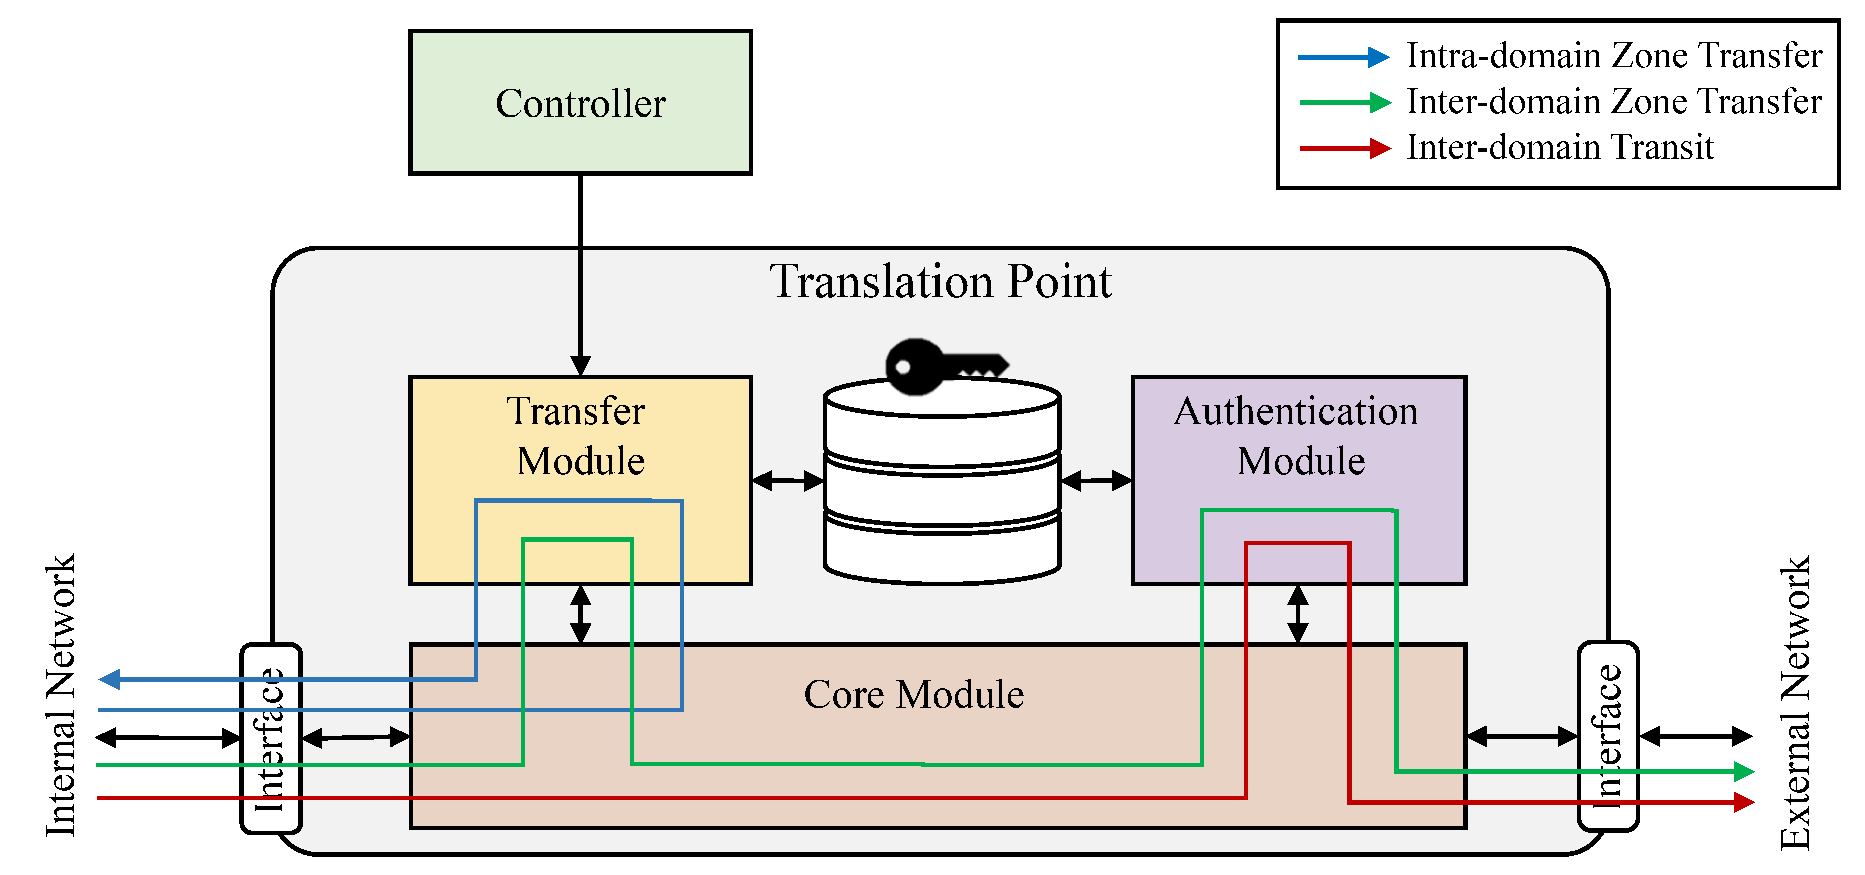
\includegraphics[width=0.9\textwidth]{tp.eps}
	\end{center}
	\caption{An overview of the modularized \tp implementation. Major usecases are also
		indicated with colored arrows.}
	\label{fig:tp}
\end{figure}

To implement a prototype of \tp, we extend the \fnurl{SCION-IP Gateway (SIG)}{https://github.com/scionproto/scion}.
The main functionality of SIG is to encapsulate legacy IP packets into SCION packets and
vice versa. In this context, a SIG acts as a gateway between an internal (legacy) network
and an external (SCION) network. Since \tp is designed as a gateway that bridges LAN
traffic over WAN---the underlying inter-domain routing protocol is not relevant here---the
functional aspects of \tp meets with what SIG provides. To be integrated with SIG, \tp
mediates between the UNIX socket and SIG socket, and performs zone transfer authorization
and verification for all incoming/outgoing packets.

\subsection{Modular Design}
\label{ssec:mod_design}

\paragraph{Packet Format}
In order to make \tps modular, all modules must agree on a common packet format on which they
operate. The packet contains the raw IP packet read from the interface, as well as metadata
that is required by the modules to perform their task. Modules can read and write all fields of the
packet. In particular they can modify the raw IP packet.
Listing~\ref{lst:packet} shows the packet format.

\begin{minipage}{\linewidth}
	\begin{lstlisting}[
		basicstyle=\footnotesize, language=golang,
		caption={\textit{The abstract packet format passed between the modules of a \tp.}},
		label=lst:packet,
	]
	// Packet contains a raw IP packet with additional meta data
	type Packet struct {
		Ingress		bool
		SrcHost 	net.IP
		DstHost 	net.IP
		RemoteTP	string
		DstZone		uint32
		RawPacket 	common.RawBytes
	}
	\end{lstlisting}
\end{minipage}

The \code{Ingress}field identifies a packet as either an ingress packet,
coming from the WAN, or an egress packet
that originated in the local network. \code{SrcHost} and \code{DstHost} reflect
the source and destination IP addresses of the packet. \code{RemoteTP} designates
the remote \tp. For an ingress packet that is the source \tp from which the packet
was received, for an egress packet it is the \tp to which the packet needs to be
forwarded to. \code{DstZone} is the Zone ID of the zone to which \code{DstHost}
belongs.

\paragraph{Module Interface}
A module is then simply defined as a type that handles this packet format.
More precisely, a module implements a very simple \code{Module} interface.

\begin{minipage}{\linewidth}
	\begin{lstlisting}[
		basicstyle=\footnotesize, language=golang,
		caption={\textit{The interface all modules must implement.}},
		label=lst:module,
	]
	// Module is a single element in the pipeline
	// that handles IP packets.
	// Modules must be thread safe.
	type Module interface {
		Handle(Packet) (Packet, error)
	}
	\end{lstlisting}
\end{minipage}

As can be seen in Listing~\ref{lst:module}, modules call \code{Handle} to process packets
of the aforementioned format and then return a new, potentially modified, packet and an
error. The error is \code{nil} if the handling of the packet was successful.

\paragraph{Handler Chains}
\label{ssec:chains}

\cmnt{TODO}

\subsection{Implemented Modules}
\label{ssec:modules}

In this section we describe the main modules that have been implemented to satisfy
the protocol described in \S\ref{sec:protocol}. Figure~\ref{fig:tp} illustrates
the implementation details of the modularized \tp design that consists of the three
main modules: i) core module, ii) transfer module, and iii) authentication module.

\paragraph{Core Module}
The core module is the main loop of \tp. It reads packets from the UNIX socket and
redistributes them to the corresponding interfaces. More precisely, when receiving packets
from the internal network, it retrieves metadata such as source and destination
IP addresses (as illustrated in
\S\ref{ssec:mod_design}) from the raw packet and hands over to the transfer module.
If the zone transfer is authorized ($return=1$),
the packet is then either forwarded back to the internal network or, in case the given destination is in a remote zone, once again handed over to the authentication module to be prepared for secure transmission.
For packets coming from the external network, \tp first calls the authentication module for
verification of the conveyed authentication token. Packets with invalid tokens are simply discarded.

\paragraph{Transfer Module}
The main objective of this module is to check the zone transfer rules. The transfer
module communicates with its controller to maintain a list of up-to-date zone transfer policies.
To this end, it establishes a TLS channel with the controller, downloads policies,
and populates the database.
We implemented the transfer module to support different drop-in options using APIs.

\begin{itemize}
	\item No-Op: This is for a setup in which no inter-domain zone transfers are required,
	      but only inter-domain zone extensions.
	\item Standard: This mode would perform an authorization check for the requested
	      zone transfer based on the source and destination IP addresses.
	\item Firewall: If needed, the module could be instantiated as a full-fledged firewall.
	      This mode would be useful for cases where the firewall can not be replaced.
	      \cmnt{should we discuss this further in the discussion section?}
\end{itemize}

\paragraph{Authentication Module}
For inter-domain packet transmissions, the authentication module issues an
authentication token for the packet. It (ideally) caches the first-level keys prefetched
from other \tps and derive a second-level key to generate the authentication token.
Inversely, for packets from other \tps, it derives the corresponding 2nd-level key
and verifies the delivered authentication token. \cmnt{explain implementation in more detail}

\begin{lstlisting}[
	basicstyle=\footnotesize, language=golang,
	caption={\textit{The KeyManager interface used to by the authentication module to fetch and
	derive keys.}},
]
// KeyManager is a thread-safe key store managing L0 and L1 keys
type KeyManager interface {
	// FetchL1Key fetches the level 1 key to be used to send
	// data to remote. It returns the key and a bool
	// indicating if the cached key was expired and a fresh
	// key has been fetched from remote.
	FetchL1Key(remote string) ([]byte, bool, error)
	// FetchL2Key fetches the Level-2 key used to encrypt
	// outgoing traffic
	FetchL2Key(remote string, zone uint32) ([]byte, bool, error)
	// Derive L1Key derives the level 1 key used to derive
	// the L2 key.
	DeriveL1Key(remote string) ([]byte, error)
	// Derive L2Key derives the level 2 key used to verify
	// incoming traffic.
	DeriveL2Key(remote string, zone uint32) ([]byte, error)
}
\end{lstlisting}

\cmnt{\paragraph{Database}
	The \tp's database consists of three tables: \textit{Zone Table}, \textit{Zone Transfer
		Table}, and \textit{Key Table}. The zone table is used to map hosts to their corresponding
	zones. For a fast table lookup, we leverage Radix Trees (also known as a trie or compact prefix
	tree), \fnurl{cidranger}{https://github.com/yl2chen/cidranger} in particular. The zone transfer table is a database
	in which the zone transfer rules are stored. The two tables are populated with the information
	acquired from the controller. The key table is where the shared first-level keys are
	accumulated.}

\section{Controller}
\label{sec:controller}

We implemented the controller as a Web server written in golang with an SQLite database storing the
zone information and transfer policies. The controller offers an API which allows
\tps to fetch zoning information via HTTPS GET requests.

\paragraph{APIs}
The endpoints of interest are:

\begin{enumerate}
	\item \code{/api/get-subnets}
	\item \code{/api/get-transfers}
\end{enumerate}

Using these endpoints \tps fetch IP subnet and zone transfer rules. Important
to note is that the controller only hands out the subset of the full set of rules
which is required for the requesting \tp to be operational. This minimizes the size
of data transmissions and also improves security by not disclosing the full network
view to every \tp. For every call to the API the controller first verifies the
authenticity of the caller before the request is forwarded to the corresponding
handler. The handlers then load the requested data from the database and send it to
the caller as JSON-formatted bytes.

\begin{minipage}{\linewidth}
	\begin{lstlisting}[
		basicstyle=\footnotesize, language=golang,
		caption={\textit{Abstraction layer function that returns the relevant subnet
		information for a given \tp.}},
		label=lst:subnets,
	]
	// GetSubnets returns all subnets stored in the backend
	// relevant for ZTP with address tpAddr.
	func (b *Backend) GetSubnets(tpAddr string)
		([]*types.Subnet, error) {
	
		stmt := `WITH tp_zones
		AS (SELECT DISTINCT zone 
			FROM   subnets 
			WHERE  tp_address = ?), 
		possible_dests 
		AS (SELECT DISTINCT dest
			FROM   transfers 
			WHERE  src IN tp_zones AND dest NOT IN tp_zones), 
		possible_src 
		AS (SELECT DISTINCT src
			FROM  transfers 
			WHERE  dest IN tp_zones AND src NOT IN tp_zones) 
		SELECT net_ip, net_mask, zone, tp_address 
		FROM   subnets 
		WHERE  zone IN tp_zones OR zone IN possible_dests
		   OR zone IN possible_src`
	
		rows, err := b.db.Query(stmt, tpAddr)
		if err != nil {
			return nil, err
		}
	
		// parts of code omitted

		return nets, nil
	}
	\end{lstlisting}
\end{minipage}

\paragraph{Database}
The database consists of four tables (Zones, Sites, Subnets, Transfers), each describing one of
the core elements of the architecture.
The database schema is listed in the Appendix~\ref{apdx:controllerdb}. An abstraction layer
written in golang allows the controller to interface with the database using high-level calls.
The abstraction layer makes use of transactional queries to ensure consistency even in the event
of errors. Furthermore, the abstraction uses prepared statements for insertions, deletions and
retrievals of data. This protects against SQL-injections and improves the speed of queries.
An example function of the abstraction layer is depicted in Listing~\ref{lst:subnets}.

\section{Authentication Token}
\label{sec:token}

\begin{figure}[htb]
	\begin{center}
		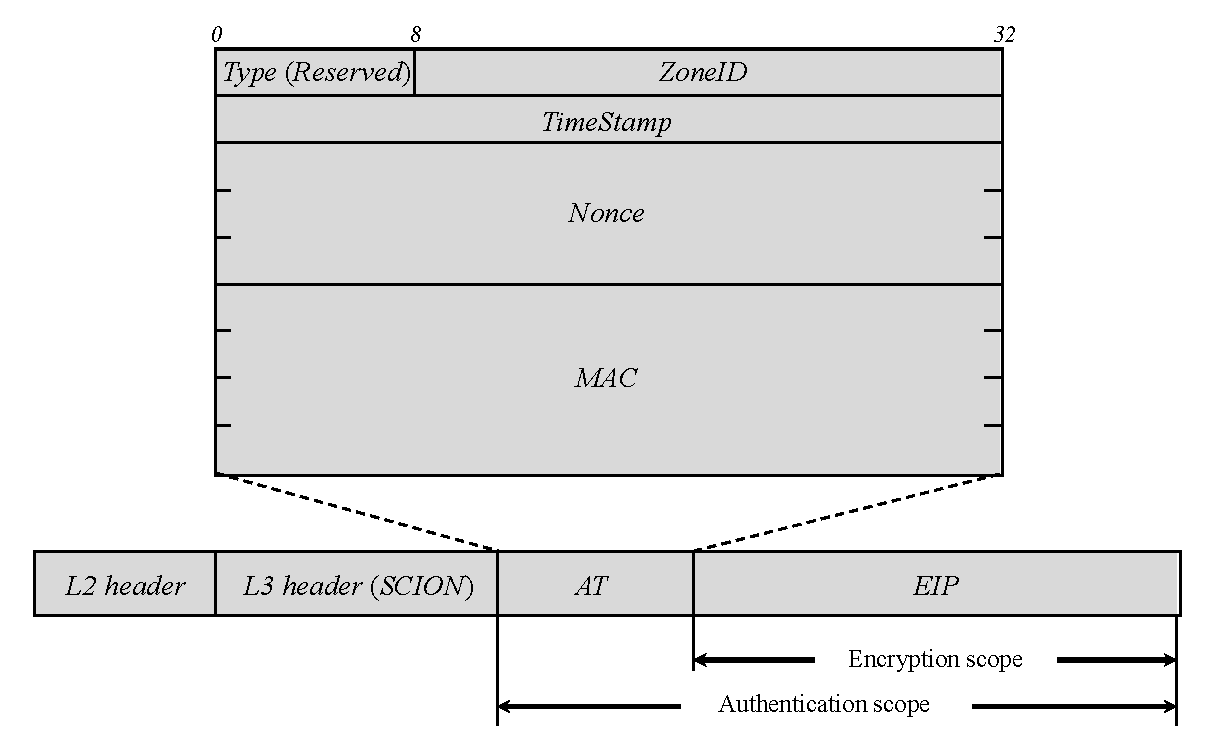
\includegraphics[width=.9\textwidth]{header.eps}
	\end{center}
	\caption{\name packet format for secure tunneling.}
	\label{fig:header}
\end{figure}

The \name packet format follows the IP tunneling conventions of encapsulating the original
packet with a new outer IP header that indicates the two tunnel endpoints as the new source
and destination. The original packet is encrypted and then authenticated along with the new
packet header fields. Figure~\ref{fig:header} shows the detailed packet structure and coverages
of the confidentiality and integrity guarantee.

The authentication token starts with one byte of reserved space for a \textit{Type} field. While
currently unused this will be useful in the future for distinguishing different variations of
the authentication token. \textit{ZoneID} depicts the 3 byte long zone identifier of the
destination zone. It is used by the receiving \tp to derive the correct key for MAC verification
and decryption. The next 4 bytes are occupied by a \textit{TimeStamp} which is added by the
sending \tp. It is the Unix time at the point of sending the packet. The receiving \tp uses this
timestamp to reject replayed packets. The timestamp is followed by a \textit{Nonce} of 12 bytes.

The nonce as well as the previous three token fields and the data to be encrypted (\textit{EIP})
serve as input to a \textit{Galois/Counter Mode} (GCM) algorithm with an underlying
\textit{AES-128} block cipher as cryptographic primitive. This mode of operation is widely
adopted for its performance as well as the capability to do \textit{authenticated encryption
	with associated data} (AEAD). Here it provides authenticity over the header fields
(\textit{Type}, \textit{ZoneID}, \textit{TimeStamp}) and the data in \textit{EIP} while
\textit{EIP} additionally also gets encrypted.

The 16 byte \textit{MAC} generated by GCM is the last field in the authentication token. Both,
the nonce and the MAC sizes follow the guidelines recommended by NIST SP 800-38D \cite{nistgcm}.

Listing~\ref{lst:transformer} shows the interface that is used by the authentication module
to create and attach an authentication token to an IP packet. Of particular interest are the
functions \code{ToIR} and \code{FromIR}. \code{ToIR} takes the raw
\code{packet}, a \code{key} and some metadata (\code{remote}, \code{dstZone}) and returns the
encrpyted packet with attached tag and an error. The error is \code{nil} if the
call was successful.
Inversely, \code{FromIR} receives an encrypted packet with attached token (\code{cipher}) and
a \code{key} and then returns the decrypted \code{packet} together with the token (\code{additionalData})
and an error. The error is again \code{nil} if the
call to the function was successful.

\begin{minipage}{\linewidth} % minipage makes the listing unsplittable
	\begin{lstlisting}[
		basicstyle=\footnotesize, language=golang,
		label={lst:transformer},
		caption={\textit{The Transformer interface used by the authentication module 
		to create and verify authentication tokens.}},
	]
	// Transformer transforms IP packets to and from intermediate
	// representation
	type Transformer interface {
		// ToIR transforms packet to intermediate
		// representation.
		ToIR(remote string, key, packet []byte, dstZone uint32)
			([]byte, error)
		// FromIR transforms cipher from intermediate representation
		// back to a regular IP packet
		FromIR(key, cipher []byte)
			(additionalData []byte, packet []byte, err error)
		// ResetState resets the nonce state for remote	
		ResetState(remote string) error
		// GetZone retrieves the zoneID encoded in token
		GetZone(token []byte) (uint32, error)
	}
	\end{lstlisting}
\end{minipage}
